%Figure list:
% Vsum vs. traditional 2D heatmap vs. juxtaposed maps
% Chart of color bins w/r/t CIELAB threshold, with iconic maps at intervals
% Process figure
% Real examples with different color maps




\newcommand{\teaserFig}{
  \teaser{
		\centering
		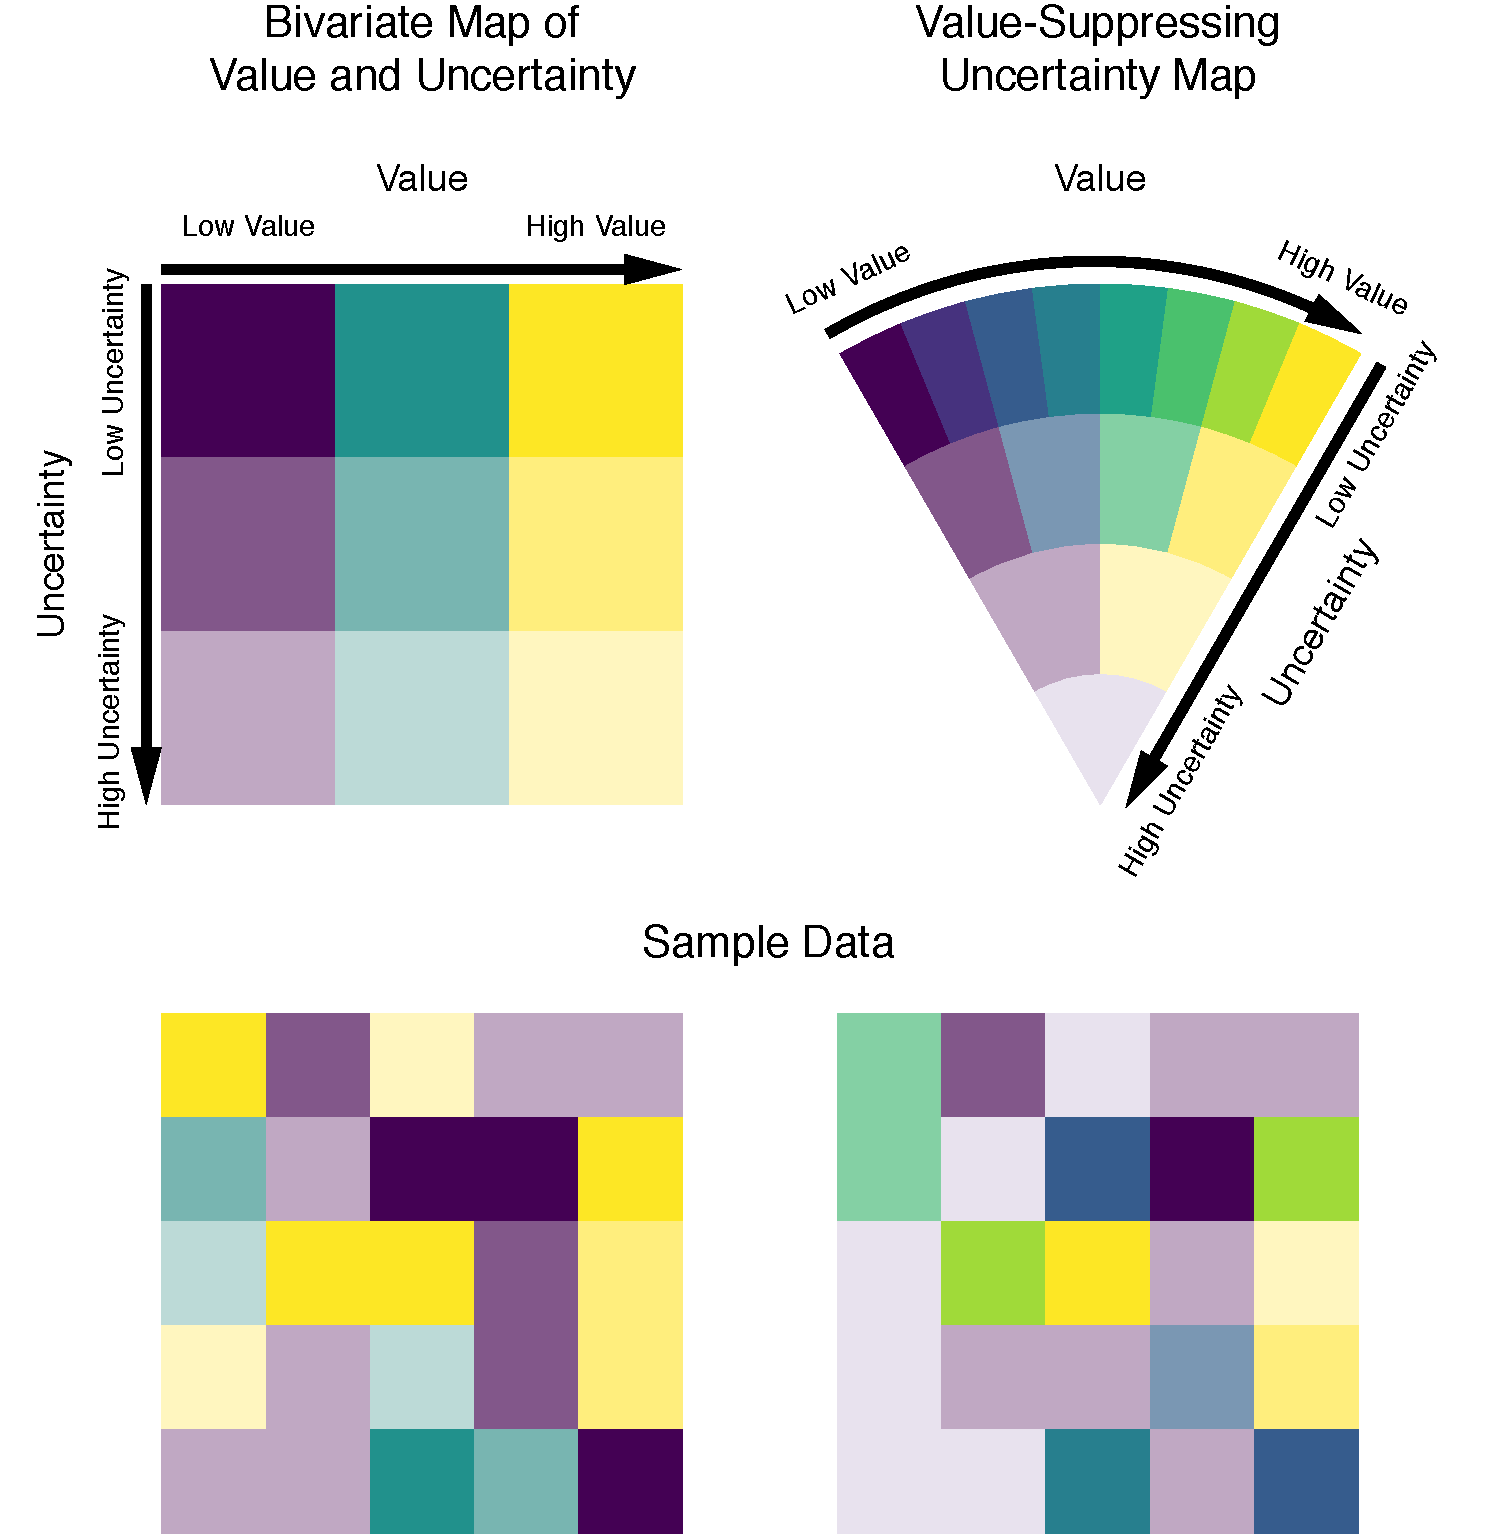
\includegraphics[width=0.9\textwidth]{example.pdf}
		\caption{Lookit! Lookit!}
		\label{fig:teaser}
	}
}

\newcommand{\exampleFig}{
\begin{figure}[t]
	\centering
	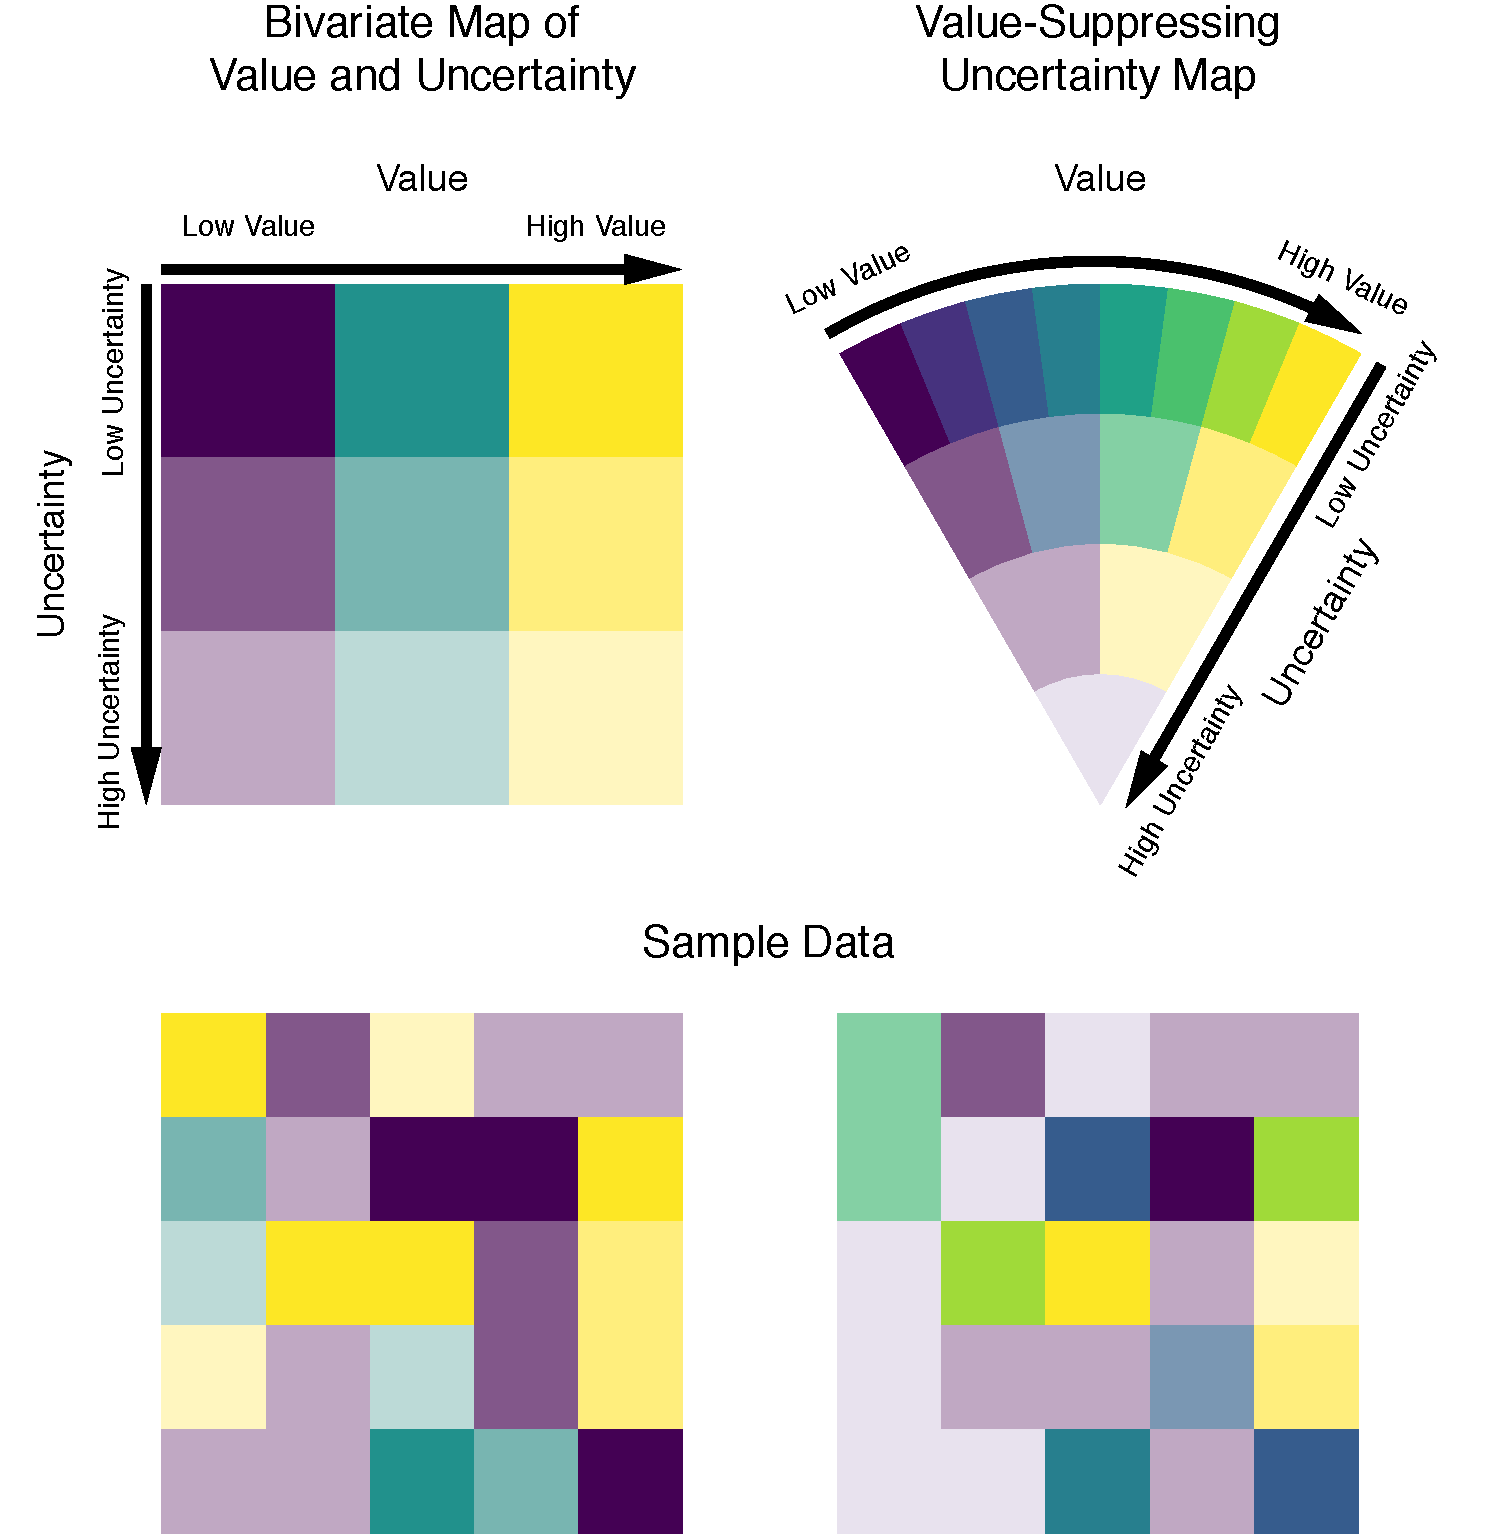
\includegraphics[width=0.9\columnwidth]{example.pdf}
	\caption{A standard bivariate map (left) and a VSUM (right), used to encode an identical 5x5 grid of random data. Both use the same visual channels to encode value (position along the Viridis~\cite{viridis} color map) and uncertainty (lightness and saturation), and have an equal standard of perceptual discriminability (at least 18 units of distance in CIELAB color space between colors). However, highly uncertain values result in colors that are very close together in the bivariate case, meaning the full bivariate map is only 9 bins under these constraints\,---\,a 4x4 map would result in colors that are perceptually too close together. By contrast, the VSUM intentionally reduces bins when uncertainty is high, eventually aliasing all highly uncertain values to the same color. This decision affords more distinct colors in other regions of the map, and so an increase in overall bins to 15. The resulting map suppresses the value of highly uncertain data, but increases the discriminability of data with low uncertainty.}
	\label{fig:example}
\end{figure}
}

\newcommand{\sizeFig}{
	\begin{figure}
		\centering
		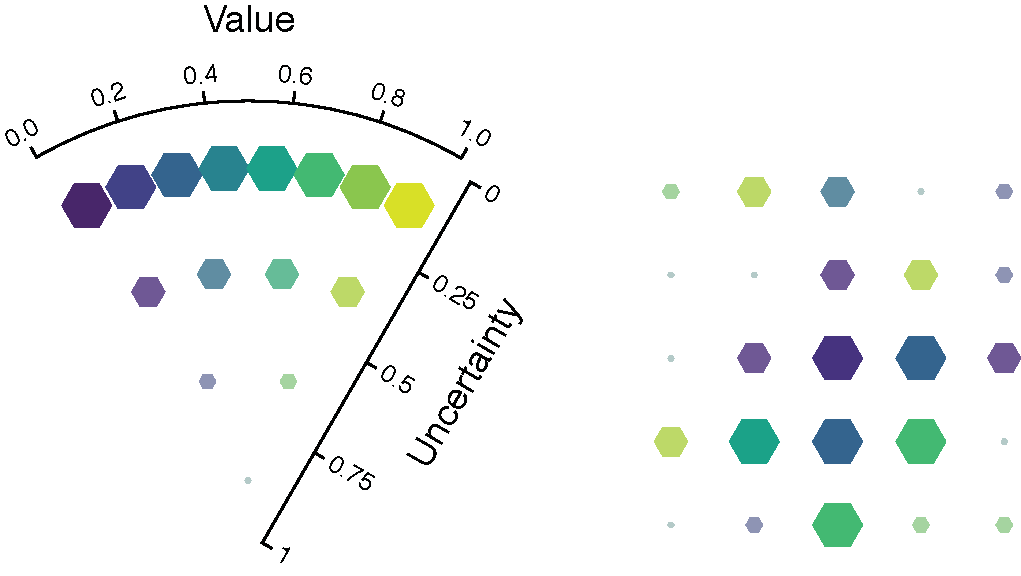
\includegraphics[width=0.9\columnwidth]{size.pdf}
		\caption{A VSUM where value is mapped to color, and uncertainty is mapped to glyph area. As glyphs become smaller, it becomes more difficult to distinguish their colors~\protect\cite{stone2014engineering}. VSUMs, by reducing the number of color categories as uncertainty increases, account for this ambiguity. On the right, the VSUM has been used to encode a 5x5 grid of random data.}
		\label{fig:size}
	\end{figure}
}

\newcommand{\conditionFig}{
	\begin{figure*}[t]
		\centering
		\begin{subfigure}{0.3\textwidth}
			\centering
			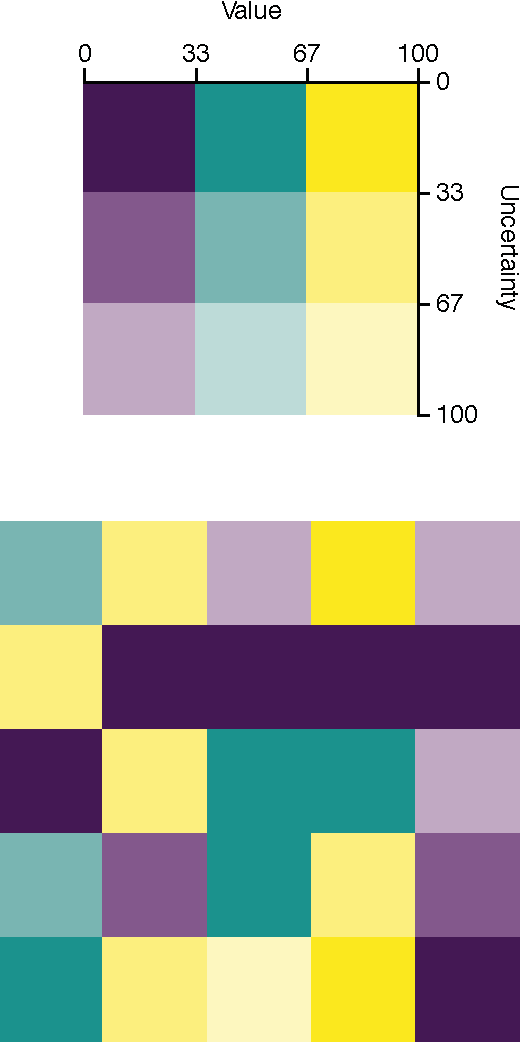
\includegraphics[width=.45\textwidth]{conditions1.pdf}
			\caption{Traditional Bivariate Map}
		\end{subfigure}
		~
		\begin{subfigure}{0.3\textwidth}
			\centering
			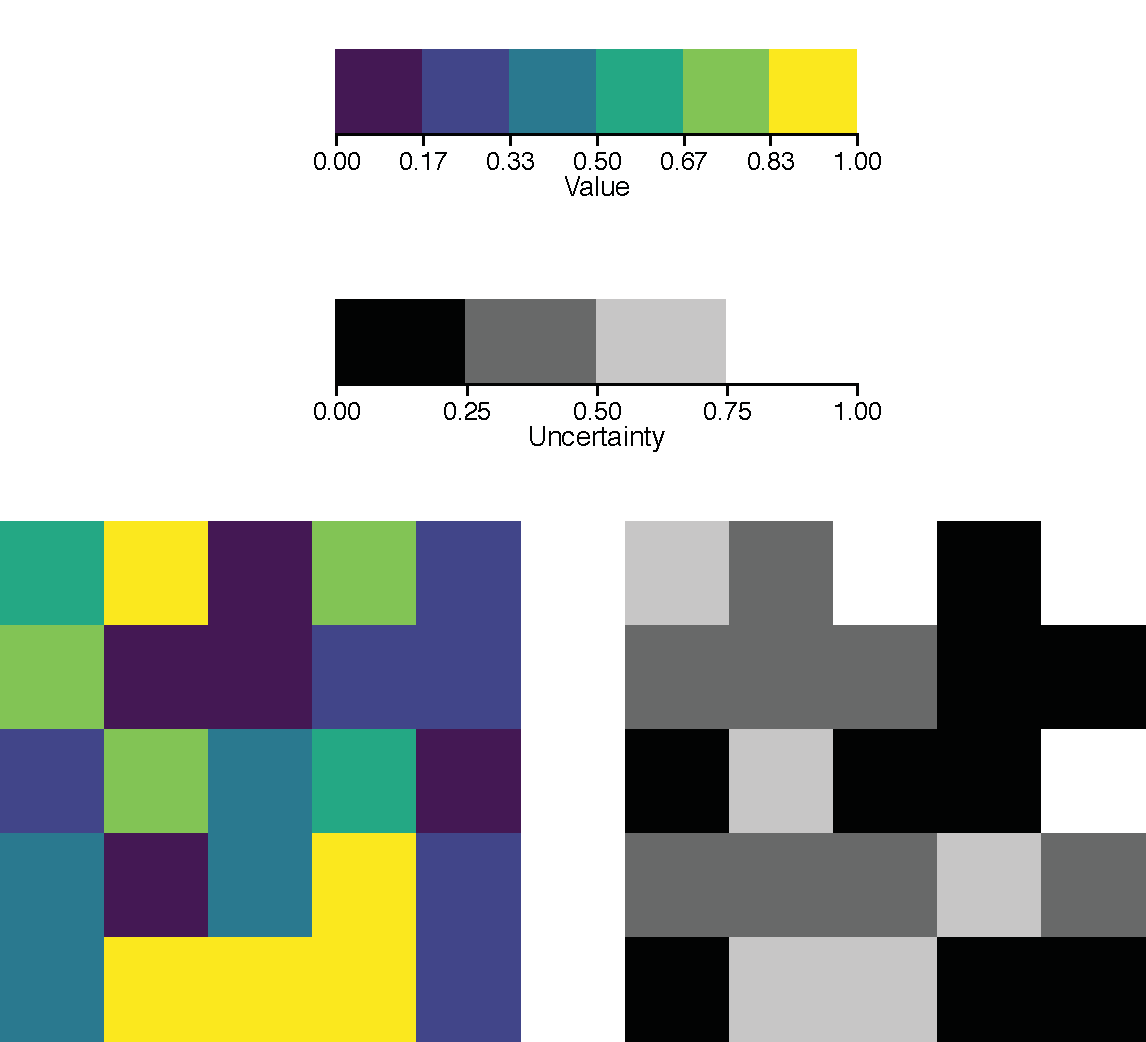
\includegraphics[width=\textwidth]{conditions2.pdf}
			\caption{Juxtaposed Univariate Maps}
		\end{subfigure}
		~
		\begin{subfigure}{0.3\textwidth}
			\centering
			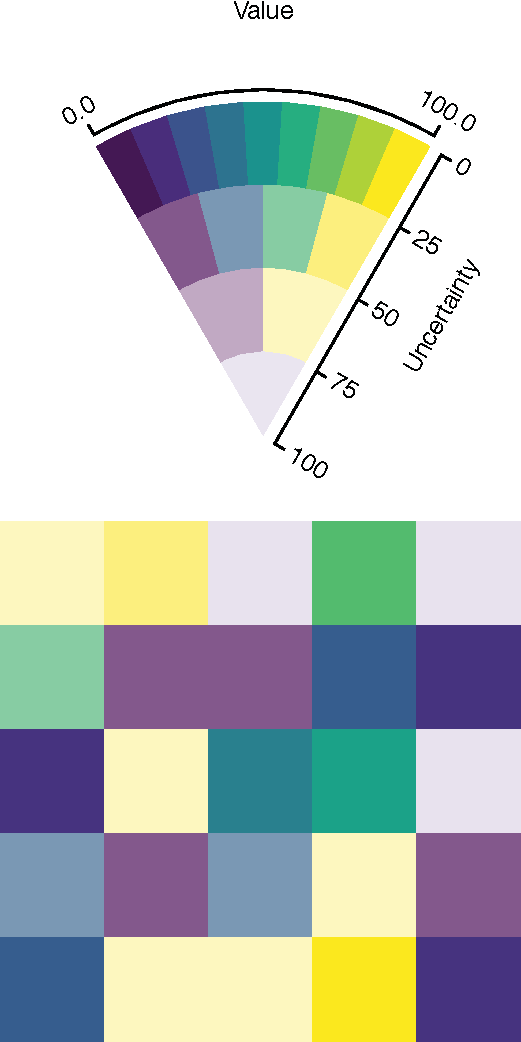
\includegraphics[width=0.45\textwidth]{conditions3.pdf}
			\caption{Value-Suppressing Uncertainty Map}
		\end{subfigure}
		\caption{The three graph types in our evaluation. Bivariate color ramps ensure that there are orthogonal mappings for each combination of value and uncertainty, but, since color channels are not separable, can afford only a few discrete colors before color categories become unacceptably close, perceptually. Juxtaposed maps, by keeping these channels separate, afford a larger range of colors, but require a visual search task to recover both value and uncertainty in a region. VSUMs have many of the advantages of bivariate maps, but assign more color categories to certain data, at the expense of ambiguity when uncertainty is high.}
		\label{fig:conditions}
	\end{figure*}
}

\newcommand{\taskTwoFig}{
	\begin{figure*}
		\centering
		\begin{subfigure}{0.45\textwidth}
			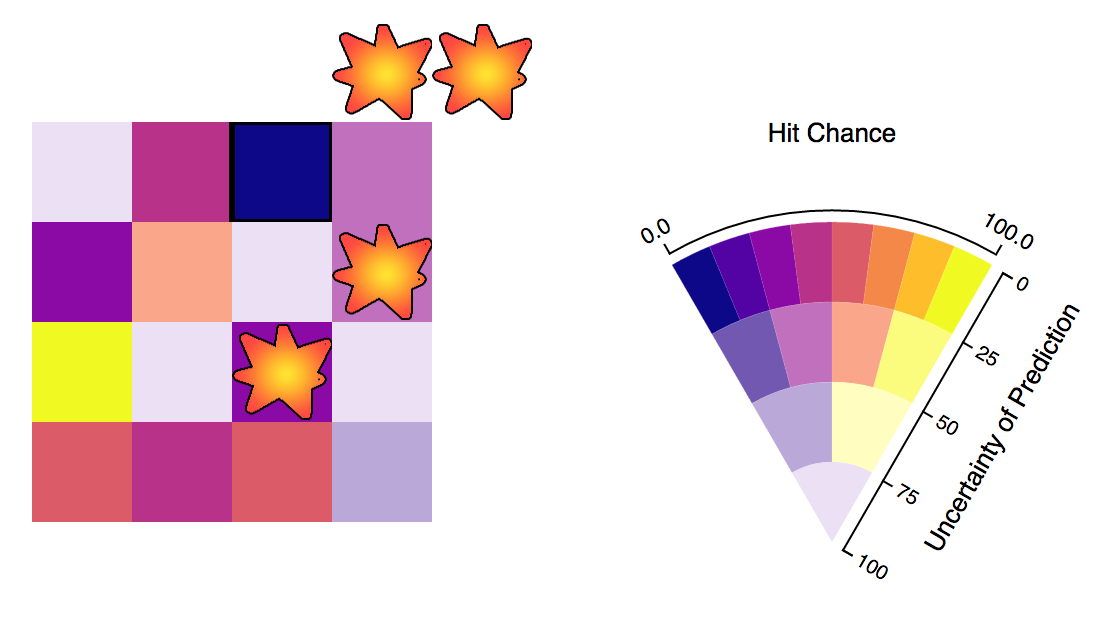
\includegraphics[width=\textwidth]{attack.png}
			\caption{Attacking}
			\label{fig:taskTwoAttack}
		\end{subfigure}
		~
		\begin{subfigure}{0.45\textwidth}
			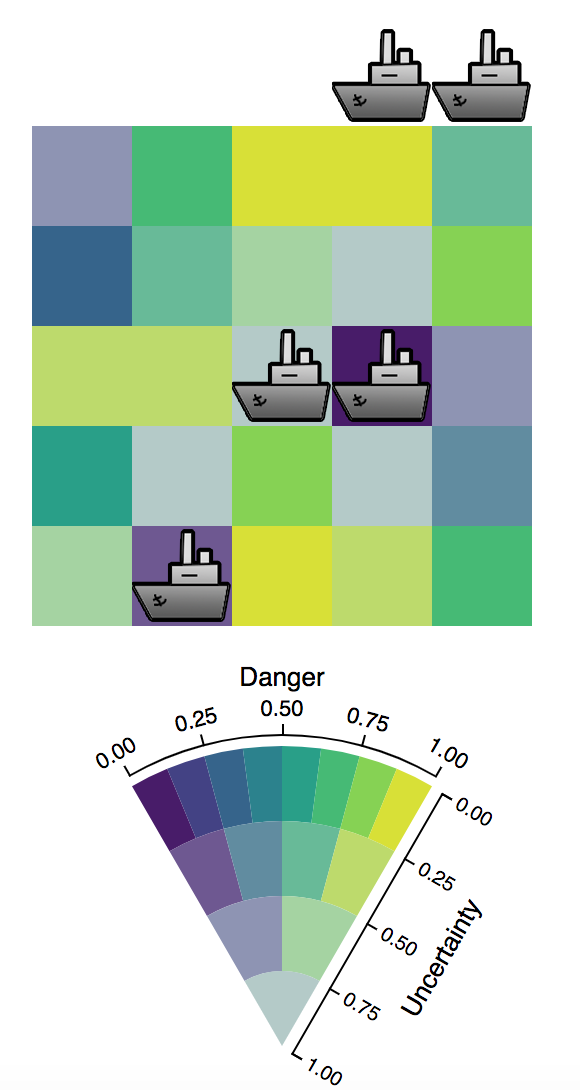
\includegraphics[width=\textwidth]{defend.png}
			\caption{Defending}
			\label{fig:taskTwoDefend}
		\end{subfigure}
		\caption{The two framings of the Prediction task. In the ``attack'' framing, the participant is given a map of predictions of the location of enemy ships, along with the uncertainty in those predictions. The participant should place their missile strikes on locations with a high probability of containing a ship, and with high certainty in this probability. The ``defend'' framing is the opposite task: the participant has a list of likely missile locations, and ought to place their ships on locations with low probability of attack, and high certainty in this probability.}
		\label{fig:taskTwoConditions}
	\end{figure*}
}

\newcommand{\performanceFig}{
	\begin{figure}[t]
		\centering
		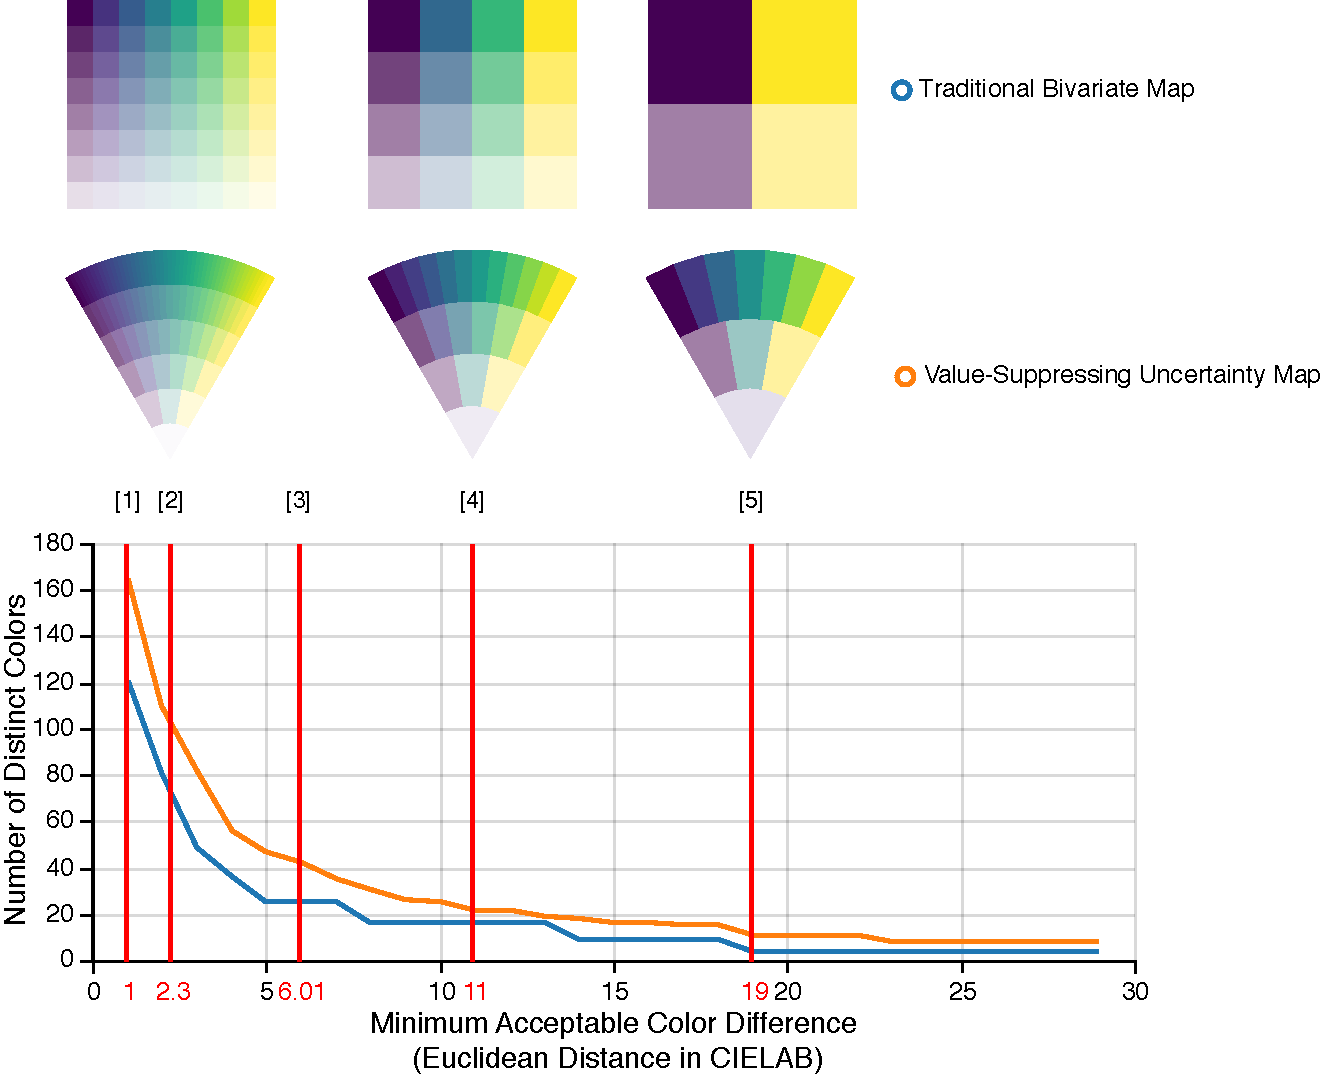
\includegraphics[width=0.9\columnwidth]{performance.pdf}
		\caption{
			The number of discrete color categories in traditional bivariate color maps versus VSUMs, assuming value is encoded by the Viridis color map~\protect\cite{viridis}, and uncertainty is encoded by saturation/value (whiter values are more uncertain). Since these whiter uncertain colors are closer together in CIELAB space, and VSUMs intentionally require fewer color bins in those regions, VSUMs always have more color categories than the corresponding 2D bivariate map. The red lines denote:
		  \textbf{1)} Theoretical 50\% JND from CIELAB specification.
			\textbf{2)} 50\% JND from controlled lab study of Mahy et al.~\protect\cite{mahy1994evaluation}.
			\textbf{3)} 50\% JND from Szafir et al.\protect\cite{szafir2014adapting}.
			\textbf{4)} 50\% JND for small visual targets from Stone et al.~\protect\cite{stone2014engineering}.
			\textbf{5)} The threshold resulting in the simplest possible (2x2) bivariate map.
	    }
		\label{fig:performance}
	\end{figure}
}

\newcommand{\flowFig}{
	\begin{figure}[t]
		\centering
		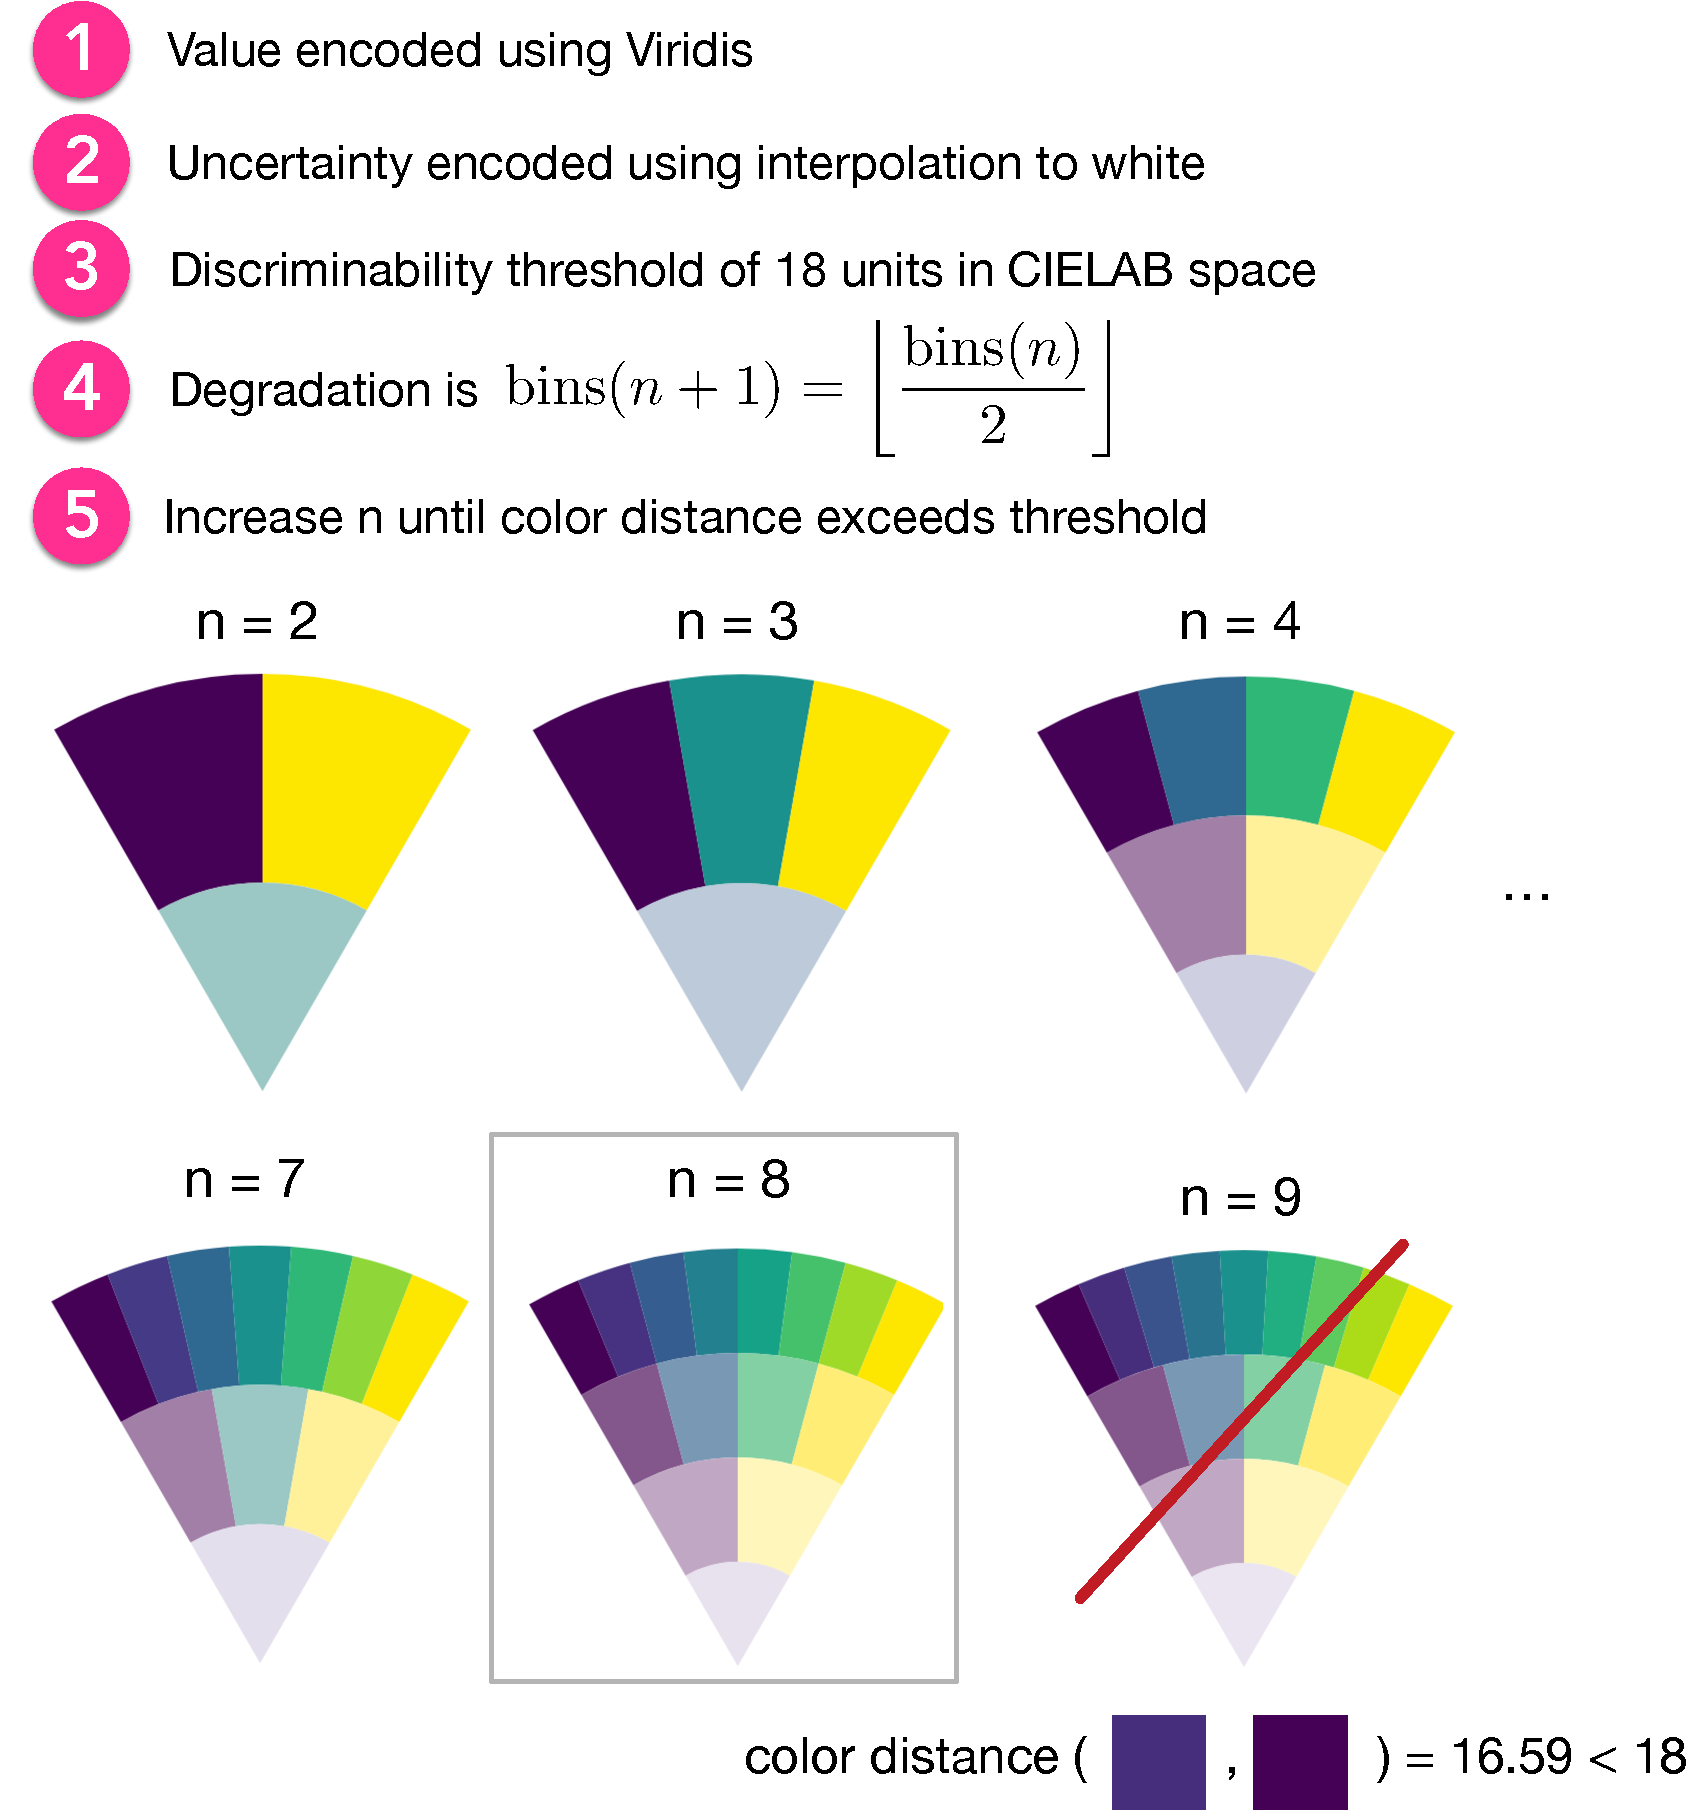
\includegraphics[width=0.95\columnwidth]{flow.pdf}
		\caption{The process for creating a VSUM. VSUMs guarantee that no two marks in the resulting bivariate mapping are perceptually closer than some pre-specified threshold. This guarantee removes some of the issues of non-separability and ambiguity that are otherwise a concern when designing bivariate maps. \\
		In this example two colors from the map for $n=9$ are too close in CIELAB space. Thus, we create a VSUM with $n=8$ color bins at the lowest level of uncertainty.}
		\label{fig:flow}
	\end{figure}
}

\newcommand{\airlineFig}{
\begin{figure}[t]
	\centering
	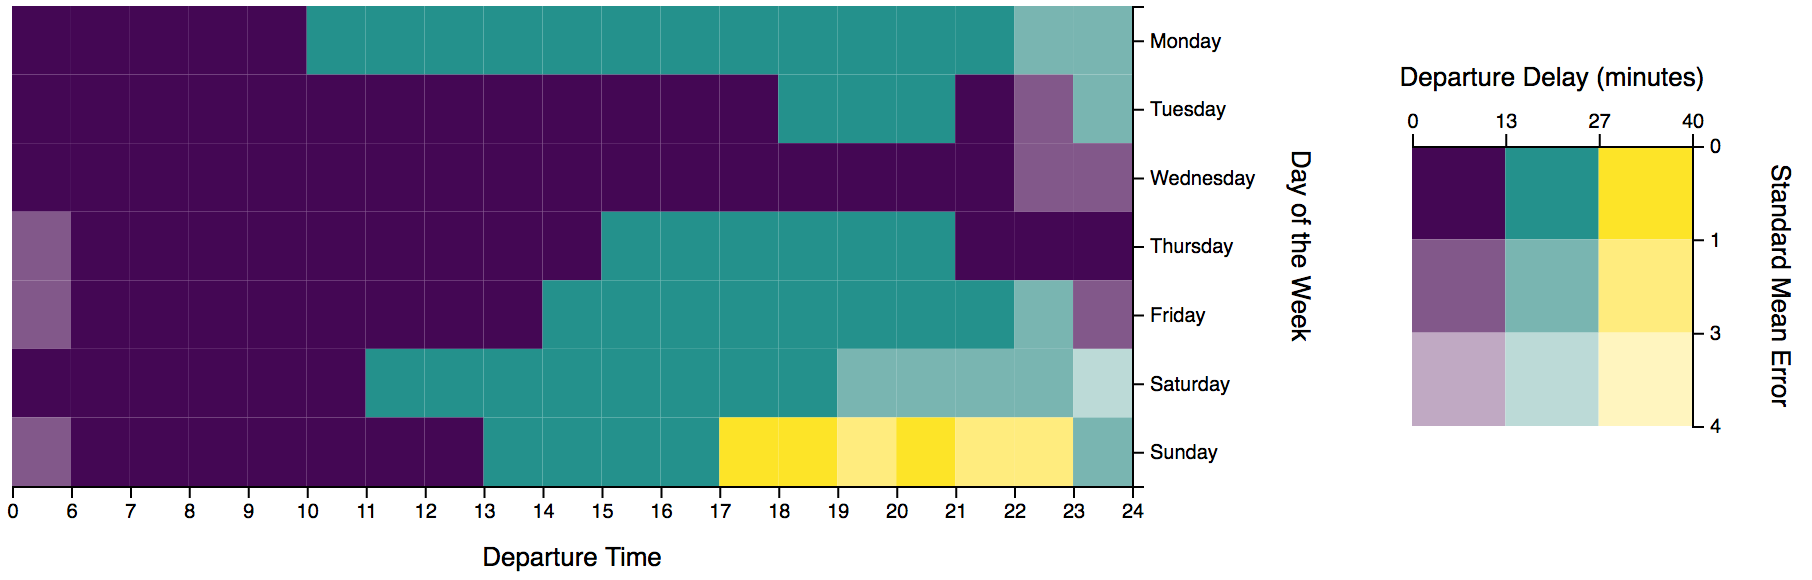
\includegraphics[width=\columnwidth]{airline-2d.png}
	\vspace{-15px}
	\caption{Average departure delay for different times of the day and days of the week visualized with a 2D uncertainty map. Horizontal position is the hour of scheduled departure, and vertical position is the day of the week.}
	\label{fig:airline2d}

	\vspace{10px}

	\centering
	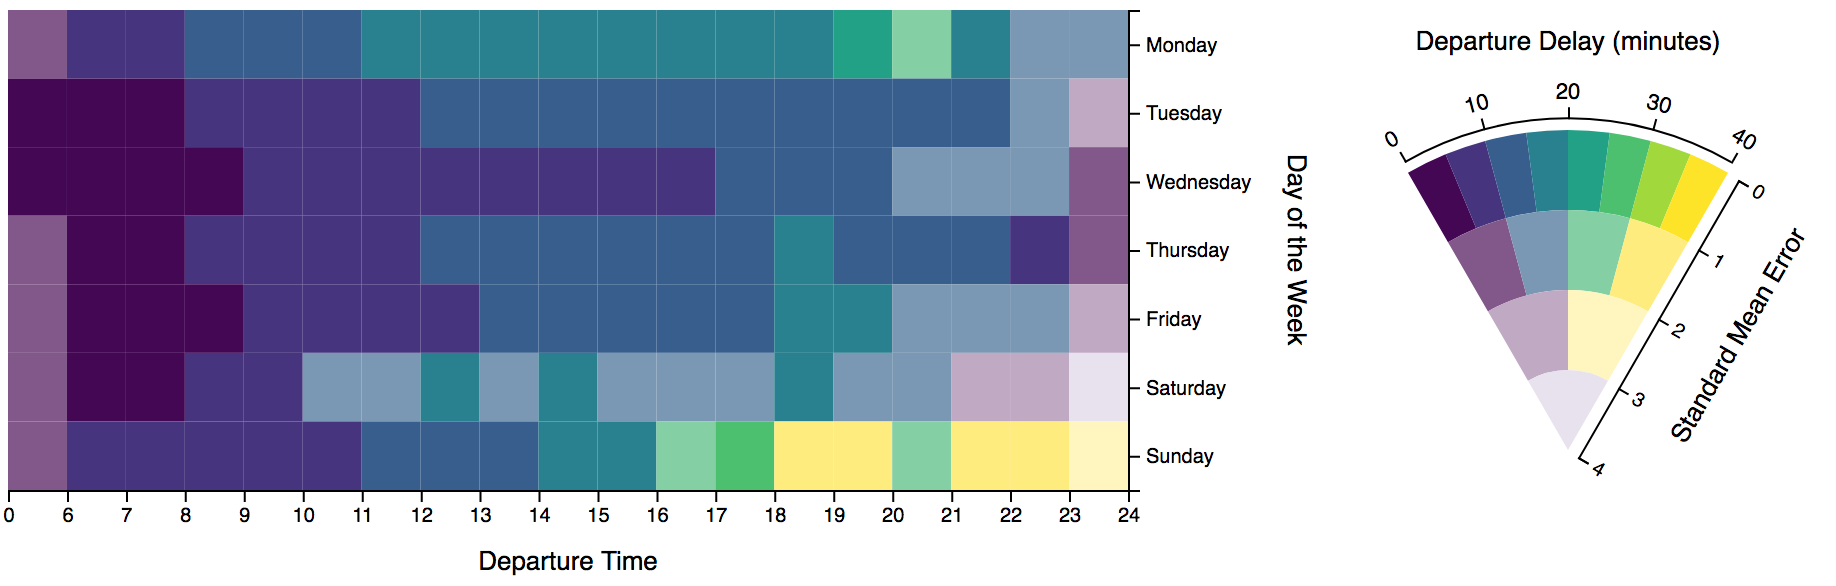
\includegraphics[width=\columnwidth]{airline-vsum.png}
	\vspace{-15px}
	\caption{Flight delay data encoded with a VSUM.}
	\label{fig:airlineVsum}
\end{figure}
}

\newcommand{\viralFig}{
\begin{figure}[t]
	\centering
	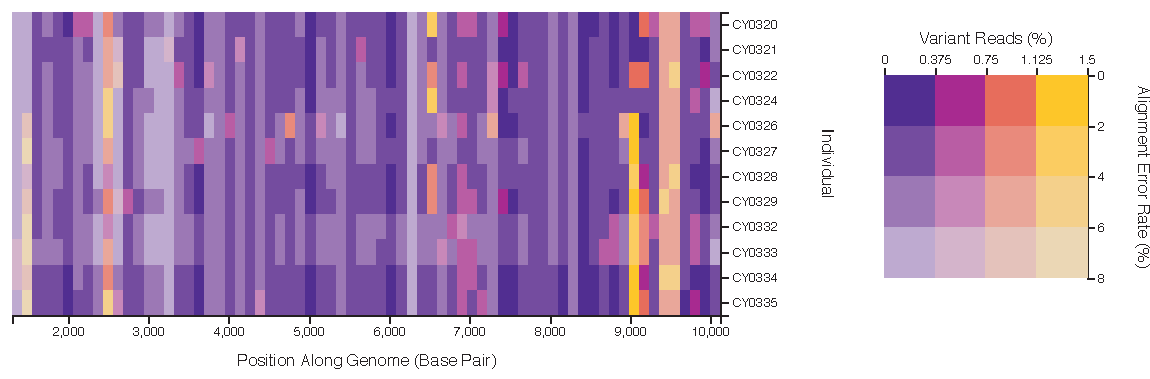
\includegraphics[width=\columnwidth]{viral-2d.pdf}
	\vspace{-15px}
	\caption{Variability for 12 different viral populations of the SIV virus, encoded with a traditional 2D bivariate map. Horizontal position denotes location along the SIV genome. Each row is the viral population of a different infected animal. Error in aligning short reads can lead to poor quality data, and so the amount of these errors is encoded as the uncertainty. }
	\label{fig:viral2d}

	\vspace{10px}

	\centering
	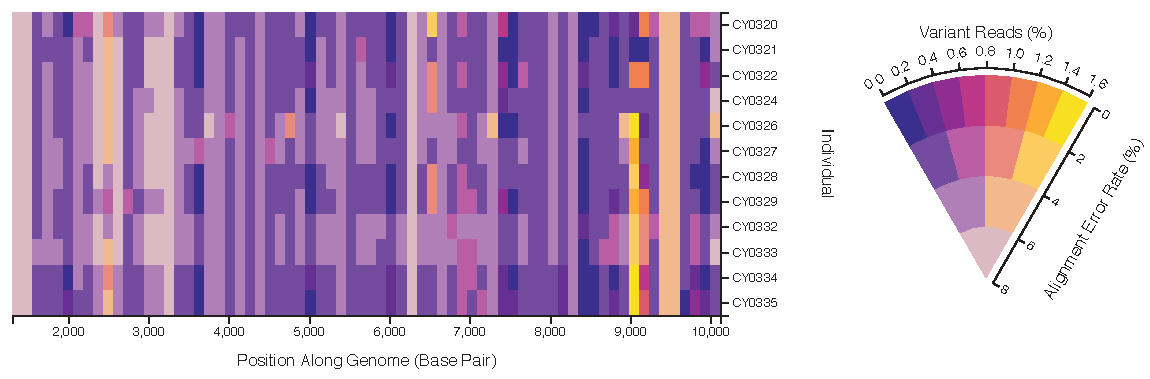
\includegraphics[width=\columnwidth]{viral-vsum.pdf}
	\vspace{-15px}
	\caption{Variability for 25 different viral populations of SIV, encoded with a VSUM. The magnitude of mutation rate, as well as the generally poorer quality of data towards the end of the sequence, is more readily visible than with the traditional bivariate color map. }
	\label{fig:viralVsum}
\end{figure}
}

\newcommand{\responseTimeFig}{
	\begin{figure}[t]
		\centering
		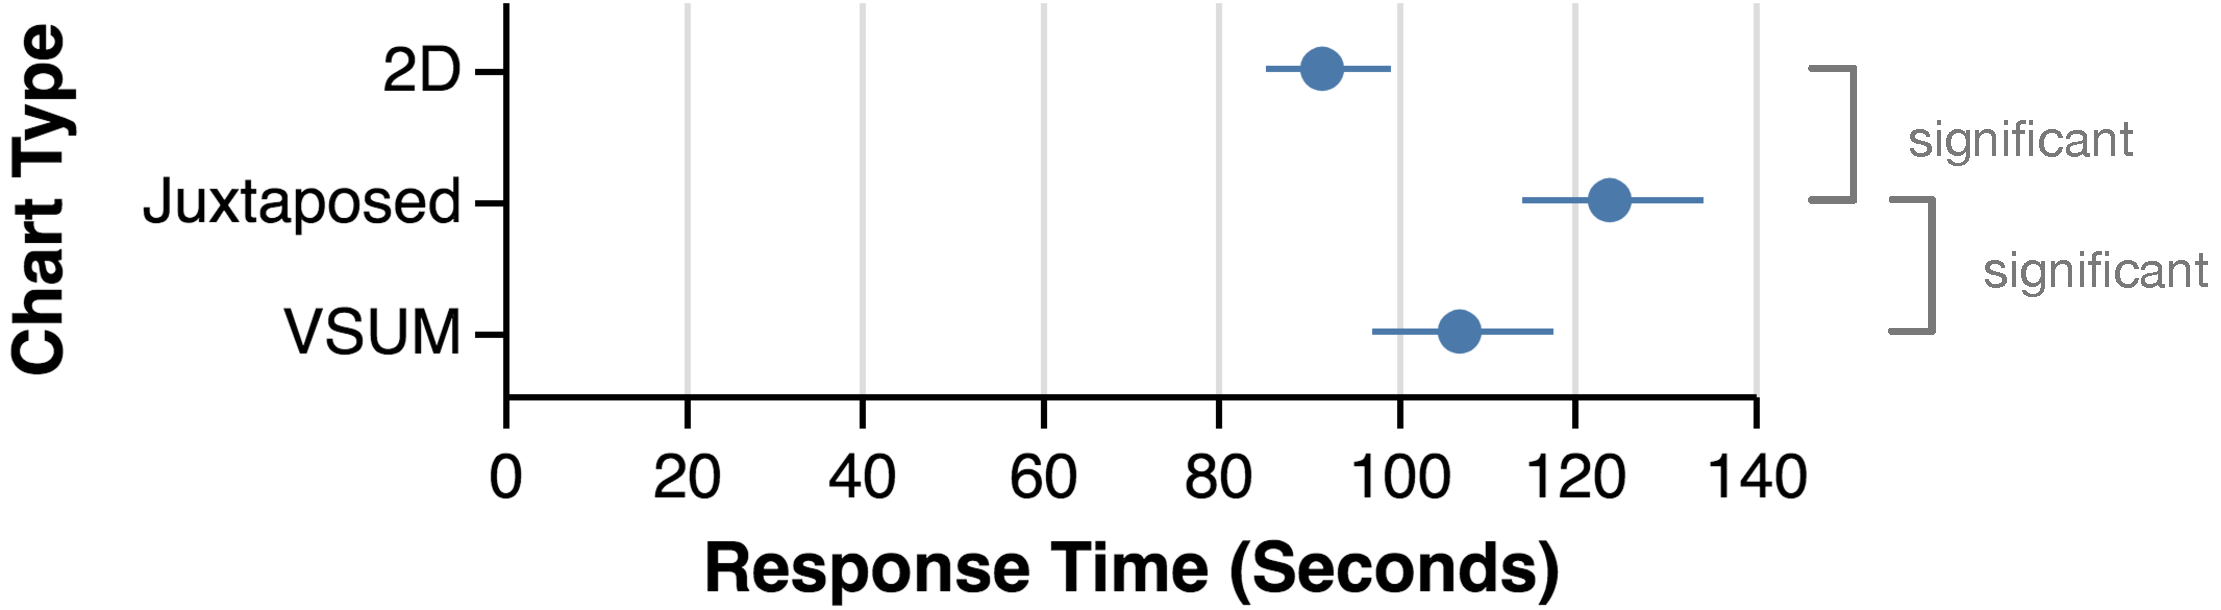
\includegraphics[height=2.4cm]{rt1.pdf}
		\caption{The effect of chart type on response time for the identification task. Juxtaposed maps of value and uncertainty introduce a visual search task, increasing the time to complete even simple tasks involving both value and uncertainty information. The confidence intervals are bootstrapped 95\% CIs of trimmed means.}
		\label{fig:rt1}
	\end{figure}
}

\newcommand{\accuracyFig}{
	\begin{figure}[t]
		\centering
		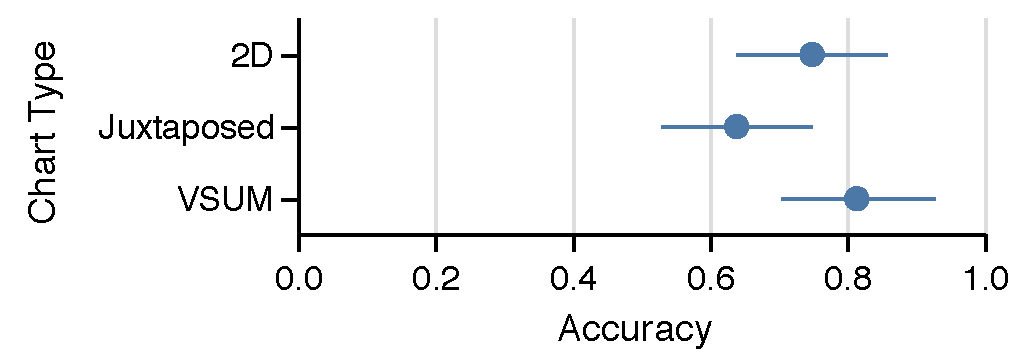
\includegraphics[height=2.4cm]{accuracy1.pdf}
		\caption{The effect of chart type on accuracy for the identification task. VSUMS are similarly accurate for simple search tasks as more traditional bivariate visualizations, despite containing additional colors categories, and having a more complex relationship between uncertainty, value, and color than traditional charts. The confidence intervals are bootstrapped 95\% CIs of trimmed means.}
		\label{fig:accuracy1}
	\end{figure}
}

\newcommand{\uncertaintyFig}{
	\begin{figure}[t]
		\centering
		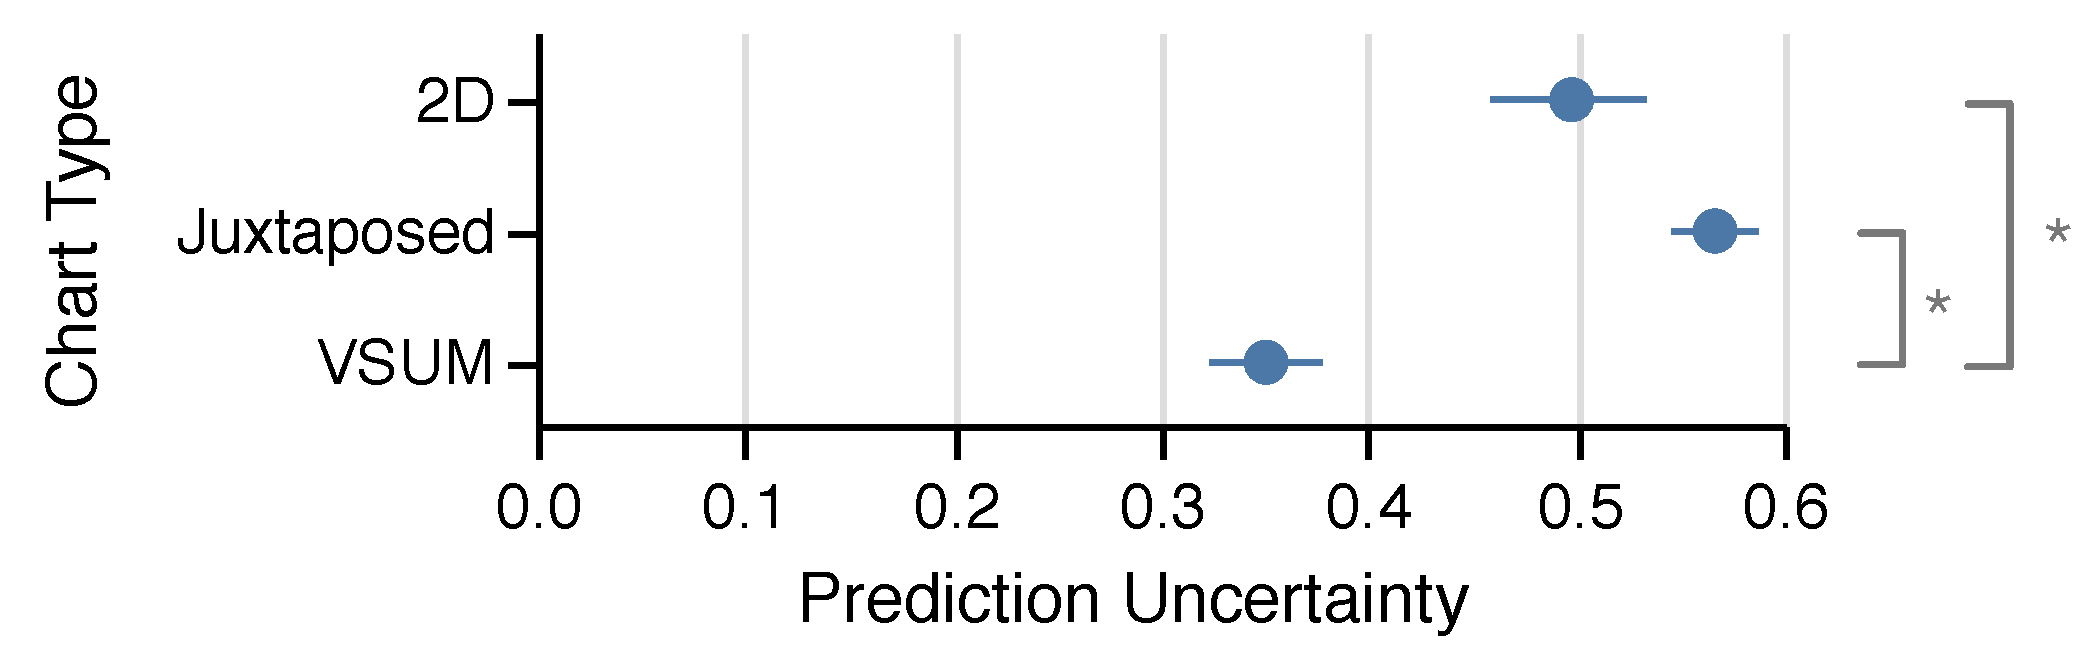
\includegraphics[height=2.4cm]{uncertainty2.pdf}
		\caption{The effect of chart type on the average uncertainty in predictions for the prediction task. By reducing the number of color categories as uncertainty increases, VSUMs encourage more caution in predictions, making people less likely to consider data with strong, but spurious patterns. The confidence intervals are bootstrapped 95\% CIs of trimmed means.}
		\label{fig:uncertainty2}
	\end{figure}
}

\newcommand{\strategyFig}{
	\begin{figure}[t]
		\centering
		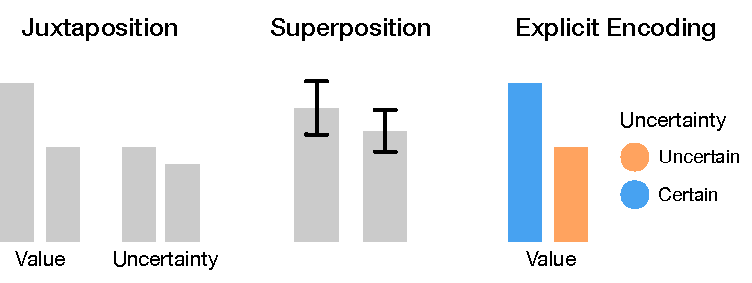
\includegraphics[width=.9\columnwidth]{strategies.pdf}
		\caption{Strategies for encoding uncertainty information along with values. From left to right: encode uncertainty as a separate visualization, overlay uncertainty information with separate glyphs in the same visualization, or encode uncertainty with a separate visual channel on the same glyphs.}
		\label{fig:strategies}
	\end{figure}
}